\chapter{Semantyka i weryfikacja programów}

Materiały teoretyczne z semantyki i weryfikacji programów zostały opracowane na podstawie \href{https://www.mimuw.edu.pl/~tarlecki/cv.pdf}{wykładu profesora Andrzeja Tarleckiego}, \href{https://www.mimuw.edu.pl/~mskrzypczak/teaching/SemWer2021/}{notatek Michała Skrzypczaka} oraz \href{https://www.mimuw.edu.pl/~czarnik/sliwowica/index.html}{seminarium SLIWOWICA}.

\section*{Podstawa programowa}
\begin{enumerate}
    \item \textbf{Metoda operacyjna} definiowania semantyki języków programowania.
    \item \textbf{Metoda denotacyjna} definiowania semantyki języków programowania.
    \item \textbf{Przekazywanie parametrów w procedurach} i reguły widoczności identyfikatorów.
    \item \textbf{Weryfikacja poprawności programów}. Metoda niezmienników. Logika Hoare'a.
\end{enumerate}

% Błażej
\section{Logika Hoare'a i dowodzenie poprawności}

\textbf{Częściowa poprawność programu} -- 
algorytm jest częściowo poprawny, gdy dla każdego zestawu danych X ze zbioru dopuszczalnych danych wejściowych, jeżeli algorytm się zatrzyma, to relacja R pomiędzy zestawem danych X, a otrzymanym zestawem wyników jest zachowana. Czyli o ile się kończy, to jesteśmy zadowoleni. Nie wiemy nic natomiast o warunku stopu. \newline
\textbf{Logika Hoare'a} to nic innego jak formalizm matematyczny służący do opisu poprawności algorytmów. Napis
$$
\{P\} \ C \ \{Q\}
$$
oznacza, że fragment kodu $C$, o ile na wejściu będzie miał stan spełniający warunek $P$ oraz \purple{o ile zakończy swoje działanie}, to na wyjściu da stan spełniający warunek $Q$. $P$ nazywamy warunkiem wstępnym, a formułę $Q$ warunkiem końcowym.
Zdefiniujmy kilka podstawowych reguł
$$
\frac{}{\{\phi\}\ \texttt{skip}\ \{\phi\}} \quad \frac{}{\{\phi[x \mapsto e ] \}\ x := e\ \{\phi\}} \quad \frac{\{\phi\}\ S_1\ \{\theta\} \ \ \{\theta\}\ S_2\ \{\psi\}}{\{\phi\}\ S_1;S_2\ \{\psi\}}
$$
$$
\frac{\{\phi \land b\}\ S_1\ \{\psi\} \ \{\phi \land \neg b\}\ S_2\ \{\psi\}}{\{\phi\}\ \texttt{if} \ b \ \texttt{then} \ S_1 \ \texttt{else} \ S_2\ \{\psi\}} \quad \frac{\{\phi \land b \}\ S_1\ \{\phi\}}{\{\phi\}\ \texttt{while} \ b \ \texttt{do} \ S\ \{\phi \land \neg b\}}
$$
$$
\frac{\phi' \Longrightarrow \phi \ \ \ \{\phi\}\ S\ \{\psi\} \ \ \ \psi \Longrightarrow \psi'}{\{\phi'\}\ S\ \{\psi'\}}
$$
Przejdźmy przez przykładowe zadanie:
\begin{example}
    \textbf{Problem:} przeprowadzić dowód poprawności częściowej programu:
    \begin{cpp}
        {n >= 1}
        x := 1; y := 0;
        while x <= n {
            y := y + x;
            x := x + 1;
        }
        {y = n(n+1)/2}
    \end{cpp}
    \textbf{Rozwiązanie:}
    \begin{enumerate}
        \item Na początek wstawmy asercję po pierwszych dwóch przypisaniach, przeciągając asercję początkową przez te przypisania
        \begin{cpp}
            {n >= 1}
            x := 1; y := 0;
            {n >= 1, x = 1, y = 0}
            while x <= n {
                y := y + x;
                x := x + 1;
            }
            {y = n(n+1)/2}
        \end{cpp}
        \item Teraz trzeba wymyślić niezmiennik pętli N taki, że
        \begin{itemize}
            \item $n \ge 1 \land x = 1 \land y = 0 \Longrightarrow N$
            \item $N \land x > n \Longrightarrow y = \frac{n(n+1)}{2}$
            \item \begin{cpp}
                {N}
                while x <= n {
                    y := y + x;
                    x := x + 1;
                }
                {N, x > n}
            \end{cpp}
        Do tej ostatniej trójki potrzebujemy
        \begin{cpp}
            {N, x <= n}
            y := y + x;
            x := x + 1;
            {N}
        \end{cpp}
        \end{itemize}
        \item Zgadujemy niezmiennik
        $$
        N = \{ y=\frac{x(x-1)}{2} \land x \le n+1 \}
        $$
        ważna sprawa -- nie zapominać o powiązaniu niezmiennika z $x$ (zadanie dla Czytelnika -- co jakby nie było fragmentu o tym, że $x\le n + 1$?)
        \item Sprawdzamy, że wszystko się zgadza.
    \end{enumerate}
    Pełne rozwiązanie:
    \begin{cpp}
        {n >= 1}
        x := 1;
        {n >= 1, x = 1}
        y := 0;
        {n >= 1, x = 1, y = 0}
        {N}
        while {N} x <= n {
            {N, x <= n}
            y := y + x;
            {y = x(x+1)/2, x <= n}
            x := x + 1;
            {N, x <= n + 1} = {N}
        }
        {y = n(n+1)/2}
    \end{cpp}
\end{example}
\textbf{Co warto zapamiętać:} należy (praktycznie zawsze) powiązać niezmiennik pętli z wartością zmiennej, od której zależy wejście do pętli. Jeśli mamy pętlę \begin{cpp}
    while (x > 0) {
        ...
        x := x - 1;
    }
\end{cpp}
i w niezmienniku nie zapiszemy warunku, że $\{x \ge 0\}$, to po wyjściu z pętli nie mamy wcale pewności, że $x=0$, a od założenia takiej właśnie wartości (w domyśle) $x$ może zależeć wartość wyrażenia po wyjściu z pętli.\newline
\textbf{Inny przykład:} rzućmy okiem na slajd z wykładu ze Wstępu do Programowania Imperatywnego autorstwa docenta Piotra Chrząstowskiego-Wachtla:
\begin{figure}[H]
    \centering
    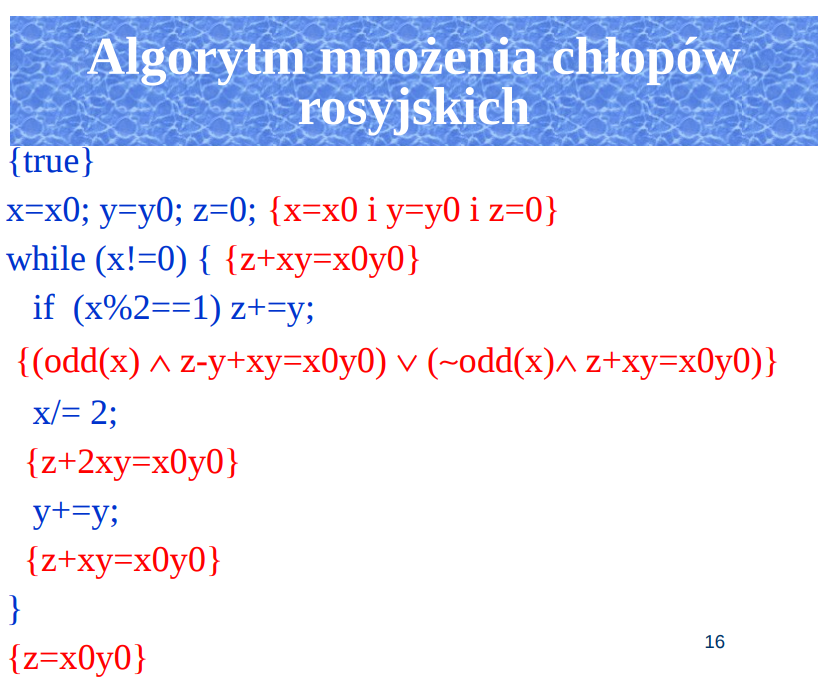
\includegraphics[scale=0.3]{rozdziały/images/CV/easter.png}
    \caption{Algorytm mnożenia chłopów rosyjskich}
\end{figure}
Napisanie trójki Hoare'a ze stanem początkowym \{\textbf{true}\} jest po prostu mega głupie.

\subsection{Pełna poprawność}
Polega na wykazaniu częściowej poprawności oraz tego, że program ma \textbf{własność stopu}. To znaczy, że dla każdych danych wejściowych zakończy działanie. Różnica między częściowo a pełną poprawnością istnieje jedynie dla instrukcji \texttt{while}. Tworząc dla niej niezmiennik musimy ustalić jakiś dobrze ufundowany porządek częściowy i dodać wielkość zmniejszającą się co obrót pętli.

\begin{example}
    \begin{cpp}
    [n >= 0]
    while [n >= 0] n > 0 do [decr n in N wrt <=] {
        n := n - 1;
    }
    [n >= 0, n <= 0]
    [n = 0]

    \end{cpp}
\end{example}

Oczywiście porządki te mogą być bardziej złożone jak np $\NN \times \NN$

\begin{example}
    \begin{cpp}
    while x > 0 do [decr (x,y) in N x N wrt <=] {
        if y > 0 then
            y := y - 1    
        else
            x := x - 1;
            y := f(x)
    }
    \end{cpp}
\end{example}

Należy zwrócić uwagę, żeby porządek był dobrze ufundowany -- czyli nie istniał nieskończony ciąg malejący, oraz żeby zawsze pozostać w tym porządku tj. jeśli piszemy: "decr $x$ in $\NN$ wrt $\leq$", to żeby $x$ nigdy nie przyjęło wartości < 0. W szczególności, kiedy rozpatrujemy porządek nad zbiorem $\NN \times \NN$ albo dowolne $\NN^k$ przyjmujemy porządek leksykograficzny po współrzędnych.

\begin{problems}
    \prob W strukturze relacyjnej, której nośnikiem jest zbiór liczb całkowitych, a wszystkie symbole operacji i~relacji mają standardowe znaczenie, następująca formuła logiki Hoare'a
    \begin{center}
        $\{x = a\}$ while $x < 0$ do $x := x \cdot a$ $\{x > 0\}$
    \end{center}
    jest prawdziwa
    \answers{dla każdego $a$}{dla każdego dodatniego $a$}{dla każdego ujemnego $a$}
    
    \prob W strukturze, której nośnikiem są liczby całkowite, prawdziwa jest trójka Hoare’a
    \answers{$\{x = y\}$ $x := x + y$ $\{x > y\}$}{$\{x = y + z\}$ if $x < y$ then $z := -z$ $\{x \leq y + z\}$}{$\{x = y \land x = z\}$ while $x > 0$ do begin $x := x - 1$; $z := z + 1$ end $\{z = 2 \cdot y\}$}
    
    \prob W strukturze liczb całkowitych zachodzi częściowa poprawność formuły logiki Hoare'a
    \answers{$\{x = y\}$ $y := y + 1$ $\{x = y + 1\}$}{$\{i \neq j\}$ if $i > j$ then $d := i - j$ else $d := j - i$ $\{d > 0\}$}{$\{x = 1\}$ while $y > x$ do $y := y - 1$ $\{y > 0\}$}

    \prob W strukturze relacyjnej, której nośnikiem jest zbiór liczb całkowitych, a wszystkie symbole operacji i~relacji mają standardowe znaczenie, formuła logiki Hoare'a
    \begin{center}
        $\{x < a\}$ while $x \neq 0$ do $x := x + 1$ $\{x = 0\}$
    \end{center}
    jest prawdziwa
    \answers{wtedy i tylko wtedy, gdy $a = 1$}{dla $a = 1$}{dla każdego $a$}

    \prob W strukturze relacyjnej, której nośnikiem jest zbiór liczb całkowitych, a wszystkie symbole operacji i~relacji mają standardowe znaczenie, formuła logiki Hoare'a
    \begin{center}
        \{\textbf{true}\} while $x > 0$ do $x := x - a$ $\{x \leq 0\}$
    \end{center}
    jest
    \answers{prawdziwa dla każdego $a$}{prawdziwa dla każdego $a > 0$}{fałszywa dla każdego $a \leq 0$}

    \prob Dany jest fragment programu wraz z warunkiem wstępnym i końcowym:
    \begin{cpp}
        // $\{s = 0 \land j = 0\}$
        while (j <= n) {
            s = s + j;
            j = j + 1;
        }
        // $\{s = \frac{n(n + 1)}{2}\}$
    \end{cpp}
    Niezmiennikiem powyższej pętli umożliwiającym wykazanie jej częściowej poprawności jest formuła
    \answers{\textbf{true}}{$s=\frac{j(j-1)}{2}\wedge j\leq n$}{$s=\frac{j(j-1)}{2}\wedge j\leq n+1$}

    \prob Rozważmy strukturę relacyjną, której nośnikiem jest zbiór liczb całkowitych, a wszystkie symbole operacji i relacji mają standardowe znaczenie. Dany jest fragment programu wraz z warunkiem wstępnym i końcowym:
    \begin{cpp}
        // $\{s = 0 \land j = n \land n > 0\}$
        while (j > 0) {
            s = s + n;
            j = j - 1;
        }
        // $\{s = n^2\}$
    \end{cpp}
    Niezmiennikiem pętli umożliwiającym wykazanie jej częściowej poprawności jest formuła
    \answers
    {$s = (n - j) \cdot n$}
    {$s = (n - j) \cdot n \wedge j \geq 0$}
    {$s = j \cdot n \wedge j \geq 0$}

    \prob Definicja formuły $\{\phi; P; \psi\}$ w logice Hoare’a mówi o tym, że
    \answers{jeśli zachodzi $\phi$, to $P$ się kończy i zachodzi $\psi$}{jeśli zachodzi $\phi$, a $P$ się kończy, to zachodzi $\psi$}{jeśli zachodzi $\psi$, a $P$ się kończy, to zachodzi $\phi$}
\end{problems}

\section{Semantyka}
Zadania prawie zawsze mają pełne przedstawienie tego czym jest środowisko ($Env$), $Store$, $Loc$, itd. Do tego dołączany jest zbiór paru regułek i krótki przykładowy program.

\subsection{Porządek zupełny}
Przydatne w zadaniach, dawka intuicji:
\begin{figure}[H]
    \centering
    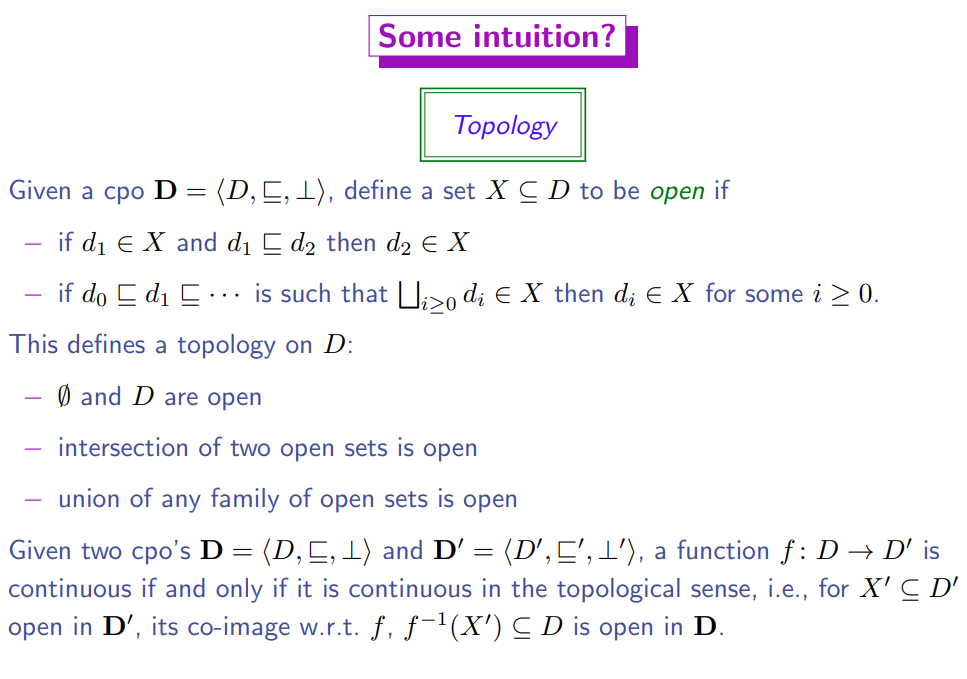
\includegraphics[scale=0.3]{rozdziały/images/CV/intuition1.png}
    \caption{Intuicja 1}
\end{figure}
\begin{figure}[H]
    \centering
    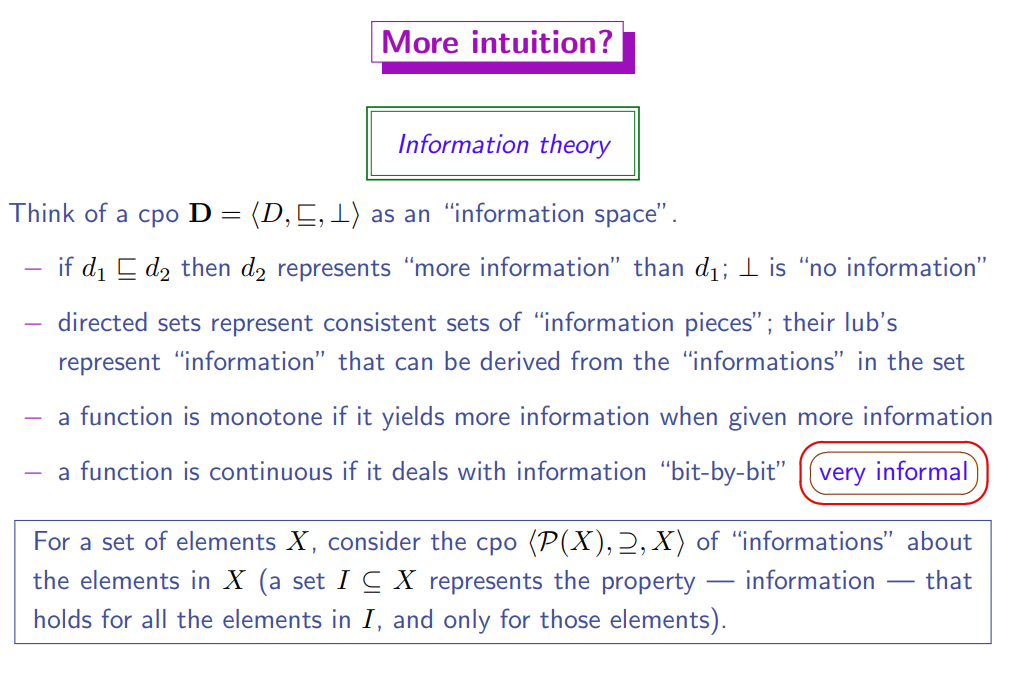
\includegraphics[scale=0.3]{rozdziały/images/CV/intuition2.png}
    \caption{Intuicja 2}
\end{figure}
\begin{figure}[H]
    \centering
    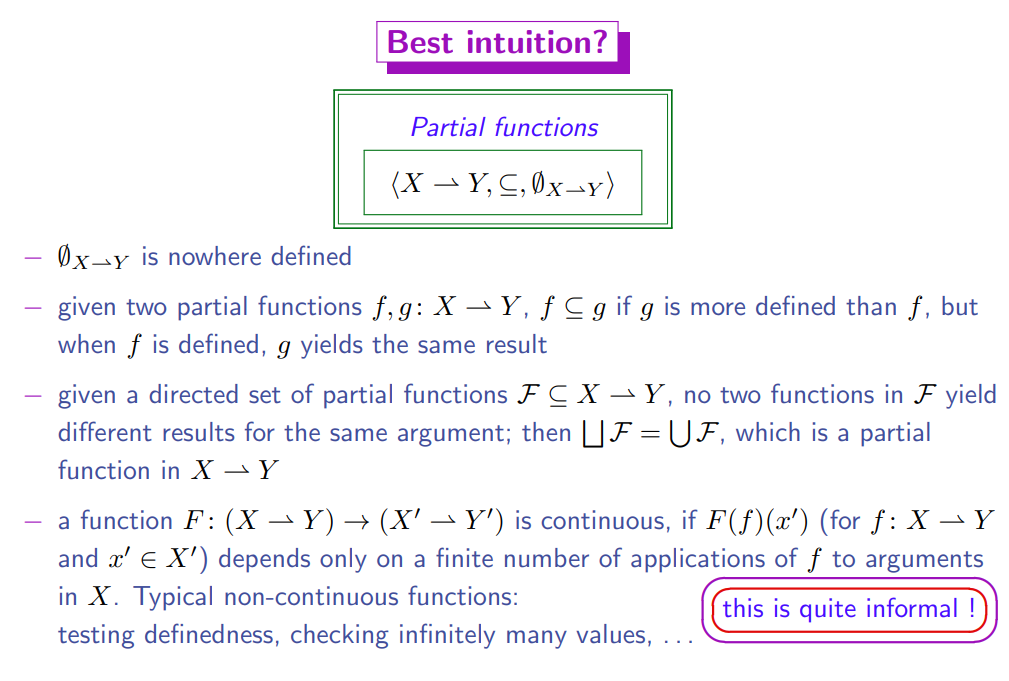
\includegraphics[scale=0.3]{rozdziały/images/CV/intuition3.png}
    \caption{Intuicja 3}
\end{figure}

\begin{problems}
    \prob Niech \textit{Ide} będzie zbiorem identyfikatorów zmiennych, a \textit{Loc} $= \{l_0, l_1, ...\}$ będzie przeliczalnym zbiorem lokacji o zadanej numeracji.
    
    Ustalmy \textit{Env = Ide} $\rightarrow$ \textit{Loc}, \textit{Store = Loc} $\rightarrow \ZZ$ oraz \textit{State = Env} $\times$ \textit{Store} $\times$ $\ZZ$, gdzie $\ZZ$ jest zbiorem liczb całkowitych.
    
    Wartością zmiennej $x \in $ \textit{Ide} w stanie $(\varrho, s, n) \in $ \textit{State} nazywamy liczbę $s(\varrho x) \in \ZZ$.
    
    Znaczenie programów definiuje funkcja semantyczna $\mathcal{P}:$ \textit{Prog} $\rightarrow$ \textit{State} $\rightarrow$ \textit{State} dana następującymi klauzulami semantycznymi:
    \begin{align*}
        \mathcal{P} \llbracket \textbf{init} \ x \rrbracket (\varrho, s, n) &= (\varrho[x \mapsto l_n], s[l_n \mapsto 0], n + 1) \\
        \mathcal{P} \llbracket \textbf{var} \ x = y \rrbracket (\varrho, s, n) &= (\varrho[x \mapsto (\varrho y)], s, n) \\
        \mathcal{P} \llbracket \textbf{inc} \ x \rrbracket (\varrho, s, n) &= (\varrho, s[(\varrho x) \mapsto (s(\varrho x) + 1)], n) \\
        \mathcal{P} \llbracket P_1; P_2 \rrbracket (\varrho, s, n) &= \mathcal{P} \llbracket P_2 \rrbracket(\mathcal{P} \llbracket P_1 \rrbracket(\varrho, s, n))
    \end{align*}
    W stanie po wykonaniu programu \texttt{
        init x;
        var y = x;
        inc y;
        inc x;
        inc y
    }
    \answers{zmienna $y$ ma wartość $3$}{zmienne $x$ i $y$ mają tę samą wartość}{zmienna $x$ ma wartość $1$}

    \prob Niech \textit{Ide} będzie zbiorem identyfikatorów zmiennych, a \textit{Loc} $= \{l_0, l_1, ...\}$ będzie przeliczalnym zbiorem lokacji o zadanej numeracji.
    
    Ustalmy $Env = Ide \to Loc, Store = Loc \to \NN$ oraz $State = Env \times Store \times \NN$.
    
    Wartością zmiennej $x \in Ide$ w stanie $(\varrho, s, n) \in State$ nazywamy liczbę $s(\varrho x) \in \NN$.
    
    Znaczenie programów definiuje funkcja semantyczna $\mathcal{P} : Prog \to State \to State$ dana następującymi klauzulami semantycznymi:
    \begin{align*}
        \mathcal{P} \llbracket \textbf{start} \ x \rrbracket (\varrho, s, n) &= (\varrho[x \mapsto l_n], s[l_n \mapsto 0], n + 1) \\
        \mathcal{P} \llbracket \textbf{inc} \ x \rrbracket (\varrho, s, n) &= (\varrho, s[(\varrho x) \mapsto (s(\varrho x) + 1)], n) \\
        \mathcal{P} \llbracket \textbf{sum}(x, y) \rrbracket (\varrho, s, n) &= (\varrho[y \mapsto l_n, x \mapsto l_n], s[l_n \mapsto (s(\varrho x) + s(\varrho y))], n + 1) \\
        \mathcal{P} \llbracket p_1; p_2 \rrbracket (\varrho, s, n) &= \mathcal{P} \llbracket P_2 \rrbracket(\mathcal{P} \llbracket P_1 \rrbracket(\varrho, s, n))
    \end{align*}
    Po wykonaniu programu \texttt{
        start x;
        inc x;
        start y;
        inc y;
        sum(x, y);
        inc x
    }
    \answers{suma wartości zmiennych $x$ i $y$ wynosi $3$}{suma wartości zmiennych $x$ i $y$ wynosi $6$}{zmienne $x$ i $y$ mają tę samą wartość}
\end{problems}

\begin{solutions}
    % Grześ
    \sol W strukturze relacyjnej, której nośnikiem jest zbiór liczb całkowitych, a wszystkie symbole operacji i~relacji mają standardowe znaczenie, następująca formuła logiki Hoare'a
    \begin{center}
        $\{x = a\}$ while $x < 0$ do $x := x \cdot a$ $\{x > 0\}$
    \end{center}
    jest prawdziwa
    \answerss{dla każdego $a$}{dla każdego dodatniego $a$}{dla każdego ujemnego $a$}{NIE}{TAK}{TAK}
    Jeśli $a$ jest dodatnie, to pętla nie wykona się i w oczywisty sposób mamy $x>0$. Jeśli $a$ jest ujemne, to pętla zrobi nam przypisanie $x=a^2$, więc zajdzie warunek $x>0$. Dla $a=0$ natomiast, pętla nie wykona się, a warunek $x>0$ jest fałszywy. Stąd formuła jest prawdziwa dla każdego $a\neq0$.

    % Grześ
    \sol W strukturze, której nośnikiem są liczby całkowite, prawdziwa jest trójka Hoare’a
    \answerss{$\{x = y\}$ $x := x + y$ $\{x > y\}$}{$\{x = y + z\}$ if $x < y$ then $z := -z$ $\{x \leq y + z\}$}{$\{x = y \land x = z\}$ while $x > 0$ do begin $x := x - 1$; $z := z + 1$ end $\{z = 2 \cdot y\}$}{NIE}{TAK}{NIE}
    Do poprawnego rozwiązania tego zadania należy wiedzieć, że liczby całkowite stanowią porządek częściowy i można je porównywać zgodnie z relacją $\le$. Dla nabrania intuicji przy okazji do porządków zupełnych warto, dla danego porządku zupełnego $D=\langle D, \sqsubseteq ,\perp \rangle$, zdefiniować zbiór $X\subseteq D$ otwarty jeśli: \begin{itemize}
        \item jeśli $d_1\in X$ oraz $d1 \sqsubseteq d_2$, to $d_2 \in X$
        \item jeśli $d_0 \sqsubseteq d_1 \sqsubseteq \dots $ taki, że $\bigsqcup_{i\ge 0}d_i\in X$, to $d_i\in X$ dla pewnego $i\ge 0$.
    \end{itemize} 
    To definiuje topologię na $D$:
    \begin{itemize}
        \item $\emptyset$ oraz $D$ są otwarte
        \item przecięcie dwóch otwartych zbiorów jest otwarte
        \item suma dowolnej rodziny otwartych zbiorów jest otwarta
    \end{itemize}
    Dla danych dwóch porządków zupełnych $D=\langle D, \sqsubseteq ,\perp \rangle$ i $D'=\langle D', \sqsubseteq' ,\perp' \rangle$, funkcja $f:D\to D'$ jest ciągła wtedy i tylko wtedy, gdy jest ciągła w topologicznym sensie. Z tą wiedzą, można przystąpić do zadania. 

    \textbf{A.} Dla $x\leq0$ formuła jest fałszywa.

    \textbf{B.} Jeżeli $x\geq y$, to instrukcja warunkowa nie wykona się i w oczywisty sposób mamy $x\leq y+z$, bo wciąż zachodzi równość. Rozpatrzmy przypadek, gdy $x<y$. Mamy na wejściu $z=x-y<0$. Instrukcja $z:=-z$ zmienia znak $-$ na $+$, więc $z>0$. Toteż, mając na początku $x<y$ i dodając liczbę dodatnią to prawej storny nierówności dostaniemy $x<y+z$, czyli w szczególności $x\leq y+z$. Formuła jest prawdziwa.

    \textbf{C.} Dla $x>0$ cośtam się dzieje, ale pomyślmy, co jeśli $x=y=z=-1$? Wtedy pętla się nie wykona, a warunek $z=2\cdot y$ jest absurdalny.

    % Grześ
    \sol W strukturze liczb całkowitych zachodzi częściowa poprawność formuły logiki Hoare'a
    \answerss{$\{x = y\}$ $y := y + 1$ $\{x = y + 1\}$}{$\{i \neq j\}$ if $i > j$ then $d := i - j$ else $d := j - i$ $\{d > 0\}$}{$\{x = 1\}$ while $y > x$ do $y := y - 1$ $\{y > 0\}$}{NIE}{TAK}{NIE}
    \textbf{A.} Gdyby po instrukcji było $\{x=y-1\}$, to byłoby dobrze, ale ponieważ tak nie jest, to jest źle.

    \textbf{B.} Jeśli Czytelnik się uważnie przyjrzy, to zobaczy, że $d=|i-j|$, gdzie $i\neq j$. Wartość bezwzględna dla liczby niezerowej jest dodatnia.

    \textbf{C.} Nie mamy żadnych wstępnych założeń co do $y$, więc przypadek $y=-69$ rozwala zadanie.

    % Grześ
    \sol W strukturze relacyjnej, której nośnikiem jest zbiór liczb całkowitych, a wszystkie symbole operacji i~relacji mają standardowe znaczenie, formuła logiki Hoare'a
    \begin{center}
        $\{x < a\}$ while $x \neq 0$ do $x := x + 1$ $\{x = 0\}$
    \end{center}
    jest prawdziwa
    \answerss{wtedy i tylko wtedy, gdy $a = 1$}{dla $a = 1$}{dla każdego $a$}{NIE}{TAK}{TAK}
    Zastanówmy się, dla jakich $x$ formuła jest prawdziwa, czyli \textbf{jeśli się kończy}, to $x=0$. Od razu widać, że dla $x<0$ pętla wyzeruje zmienną $x$. W oczywisty sposób $x=0$ również spełnia formułę. Co z $x>0$? Otóż pętla będzie działać w nieskończoność, więc formuła jest prawdziwa również w takim przypadku. Wniosek z tego taki, że jakiegokolwiek $a$ nie wybierzemy, formuła na pewno będzie spełniona.

    % Grześ
    \sol W strukturze relacyjnej, której nośnikiem jest zbiór liczb całkowitych, a wszystkie symbole operacji i~relacji mają standardowe znaczenie, formuła logiki Hoare'a
    \begin{center}
        \{\textbf{true}\} while $x > 0$ do $x := x - a$ $\{x \leq 0\}$
    \end{center}
    jest
    \answerss{prawdziwa dla każdego $a$}{prawdziwa dla każdego $a > 0$}{fałszywa dla każdego $a \leq 0$}{TAK}{TAK}{NIE}
    Do lepszego zrozumienia formuły \{\textbf{true}\}, warto rozpatrzeć funkcje częściowe $\langle X\rightharpoonup Y,\subseteq,\emptyset_{X\rightharpoonup Y}\rangle$ takie, że:
    \begin{itemize}
        \item $\emptyset_{X\rightharpoonup Y}$ nie jest nigdzie zdefiniowana
        \item dla dwóch funkcji częściowych $f,g:X\rightharpoonup Y$, $f\subseteq g$, jeśli $g$ jest bardziej zdefiniowana niż $f$, ale gdy $f$ jest zdefiniowana, $g$ produkuje taki sam wynik
        \item dla skierowanego zbioru funkcji częściowych $\mathcal{F}\subseteq X\rightharpoonup Y$, żadne dwie funkcje w $\mathcal{F}$ nie produkują różnych wyników dla tych samych argumentów; wtedy $\bigsqcup\mathcal{F}=\bigcup\mathcal{F}$, co jest funkcją częściową w $X\rightharpoonup Y$
        \item funkcja $F:(X\rightharpoonup Y)\to(X'\rightharpoonup Y')$ jest ciągła, jeśli $F(f)(x')$ (dla $f:X\rightharpoonup Y$ i $x'\in X'$) zależy tylko od skończonej liczby aplikacji funkcji $f$ do argumentów z $X$. Typowe nieciągłe funkcje: testowanie zdefiniowania, sprawdzanie nieskończenie wiele wartości, itp.
    \end{itemize}
    Z tą intuicją możemy kontynuować rozwiązanie zadania. Pomyślmy, dla jakich $a$ formuła jest prawdziwa, czyli \textbf{jeśli pętla się zatrzyma}, to spełnione będzie $x\leq0$. W oczywisty sposób widzimy, że dla $a>0$ jest to prawda. Widzimy też, że gdy $a=0$ lub też $a<0$, to pętla nigdy nie się nie skończy. Wynika stąd, że formuła jest prawdziwa dla każdego $a$, toteż odpowiedzi takie, a nie inne.

    % Grześ
    \sol Dany jest fragment programu wraz z warunkiem wstępnym i końcowym:
    \begin{cpp}
        // $\{s = 0 \land j = 0\}$
        while (j <= n) {
            s = s + j;
            j = j + 1;
        }
        // $\{s = \frac{n(n + 1)}{2}\}$
    \end{cpp}
    Niezmiennikiem powyższej pętli umożliwiającym wykazanie jej częściowej poprawności jest formuła
    \answerss{\textbf{true}}{$s=\frac{j(j-1)}{2}\wedge j\leq n$}{$s=\frac{j(j-1)}{2}\wedge j\leq n+1$}{NIE}{NIE}{TAK}
    \textbf{A.} xD

    \textbf{B.} Mając zanegowany warunek pętli $j>n$ oraz niezmiennik $j\leq n$ widzimy, że coś tu nie gra.

    \textbf{C.} Zanegowany warunek pętli $j>n$ oraz warunek z niezmiennika $j\leq n+1$ dają nam $j=n+1$, co podstawiając do wzoru dla $s$ daje $s=\frac{(n+1)(n+1-1)}{2}=\frac{n(n+1)}{2}$. Sprawdzamy też, że ów warunek jest prawdziwy przy pierwszym obrocie pętli, gdyż $0=s=\frac{0\cdot(-1)}{2}=0$, więc niezmiennik jest maśniutki. \grey{(zakładamy, że mamy warunek $n\geq0$, inaczej zadanie nie miałoby sensu)}

    % Grześ
    \sol Rozważmy strukturę relacyjną, której nośnikiem jest zbiór liczb całkowitych, a wszystkie symbole operacji i relacji mają standardowe znaczenie. Dany jest fragment programu wraz z warunkiem wstępnym i końcowym:
    \begin{cpp}
        // $\{s = 0 \land j = n \land n > 0\}$
        while (j > 0) {
            s = s + n;
            j = j - 1;
        }
        // $\{s = n^2\}$
    \end{cpp}
    Niezmiennikiem pętli umożliwiającym wykazanie jej częściowej poprawności jest formuła
    \answerss
    {$s = (n - j) \cdot n$}
    {$s = (n - j) \cdot n \wedge j \geq 0$}
    {$s = j \cdot n \wedge j \geq 0$}
    {NIE}{TAK}{NIE}
    Po pierwsze, w naszym niezmienniku musi znaleźć się reguła $j\geq0$, żeby po wyjściu z pętli, wraz z zanegowanym warunkiem pętli $j\leq0$ dostać $j=0$. Odpowiedź \textbf{A.} odpada. Podpunkt \textbf{C.} również nie ma sensu, ponieważ wiedząc, że $j=0$ dostalibyśmy $s=0\cdot n=0$. Zostaje odpowiedź \textbf{B.}, która jest poprawna, gdyż niezmiennik na początku jest spełniony ($s=0=(n-n)\cdot n$), a na koniec wraz z $j=0$ dostaniemy $s=(n-0)\cdot n=n^2$.

    % Grześ
    \sol Definicja formuły $\{\phi; P; \psi\}$ w logice Hoare’a mówi o tym, że
    \answerss{jeśli zachodzi $\phi$, to $P$ się kończy i zachodzi $\psi$}{jeśli zachodzi $\phi$, a $P$ się kończy, to zachodzi $\psi$}{jeśli zachodzi $\psi$, a $P$ się kończy, to zachodzi $\phi$}{NIE}{TAK}{NIE}
    Wprost z definicji trójki Hoare'a (odsyłam do \href{https://moodle.mimuw.edu.pl/pluginfile.php/92777/mod_resource/content/1/PoprawnoscHoareC.pdf}{slajdów docenta Piotra Chrząstowskiego-Wachtla} ze Wstępu do Programowania Imperatywnego).

    % Grześ
    \sol Niech \textit{Ide} będzie zbiorem identyfikatorów zmiennych, a \textit{Loc} $= \{l_0, l_1, ...\}$ będzie przeliczalnym zbiorem lokacji o zadanej numeracji.
    
    Ustalmy \textit{Env = Ide} $\rightarrow$ \textit{Loc}, \textit{Store = Loc} $\rightarrow \ZZ$ oraz \textit{State = Env} $\times$ \textit{Store} $\times$ $\ZZ$, gdzie $\ZZ$ jest zbiorem liczb całkowitych.
    
    Wartością zmiennej $x \in $ \textit{Ide} w stanie $(\varrho, s, n) \in $ \textit{State} nazywamy liczbę $s(\varrho x) \in \ZZ$.
    
    Znaczenie programów definiuje funkcja semantyczna $\mathcal{P}:$ \textit{Prog} $\rightarrow$ \textit{State} $\rightarrow$ \textit{State} dana następującymi klauzulami semantycznymi:
    \begin{align*}
        \mathcal{P} \llbracket \textbf{init} \ x \rrbracket (\varrho, s, n) &= (\varrho[x \mapsto l_n], s[l_n \mapsto 0], n + 1) \\
        \mathcal{P} \llbracket \textbf{var} \ x = y \rrbracket (\varrho, s, n) &= (\varrho[x \mapsto (\varrho y)], s, n) \\
        \mathcal{P} \llbracket \textbf{inc} \ x \rrbracket (\varrho, s, n) &= (\varrho, s[(\varrho x) \mapsto (s(\varrho x) + 1)], n) \\
        \mathcal{P} \llbracket P_1; P_2 \rrbracket (\varrho, s, n) &= \mathcal{P} \llbracket P_2 \rrbracket(\mathcal{P} \llbracket P_1 \rrbracket(\varrho, s, n))
    \end{align*}
    W stanie po wykonaniu programu \texttt{
        init x;
        var y = x;
        inc y;
        inc x;
        inc y
    }
    \answerss{zmienna $y$ ma wartość $3$}{zmienne $x$ i $y$ mają tę samą wartość}{zmienna $x$ ma wartość $1$}{TAK}{TAK}{NIE}
    Po wykonaniu pierwszych dwóch instrukcji mamy mapowania $x\mapsto l_0\mapsto 0$ oraz $y\mapsto l_0\mapsto 0$. W celu kontynuowania naszego rozumowania, pomyślmy o porządku zupełnym $D=\langle D,\sqsubseteq,\perp\rangle$ jako o przestrzeni informacyjnej:
    \begin{itemize}
        \item jeśli $d_1\sqsubseteq d_2$, to $d_2$ reprezentuje ,,więcej informacji" niż $d_1$; $\perp$ oznacza brak informacji
        \item zbiory skierowane reprezentują spójny zbiór ,,kawałków informacji"; ich lub-y reprezentują ,,informacje", które mogą być odziedziczone po ,,informacjach" ze zbioru
        \item funkcja jest monotoniczna, jeśli daje więcej informacji, gdy dostaje więcej informacji
        \item funkcja jest ciągła, jeśli przetwarza informacje "bit po bicie"
    \end{itemize}
    Dla zbioru elementów $X$, rozważmy porządek zupełny $\langle\mathcal{P}(X),\supseteq,X\rangle$ ,,informacji" o elementach w $X$ (zbiór $I\subseteq X$ reprezentuje własność --- informację --- która zachodzi dla wszystkich elementów w $I$ i tylko dla tych elementów). Z tą intuicją łatwo widać, że \texttt{inc x} i \texttt{inc y} będą zwiększać wartość pod $l_0$, na które wskazują obydwie zmienne. Także na koniec programu dostaniemy mapowania $x\mapsto l_0\mapsto 3$ oraz $y\mapsto l_0\mapsto 3$, z czego od razu wynikają odpowiedzi.

    \sol Niech \textit{Ide} będzie zbiorem identyfikatorów zmiennych, a \textit{Loc} $= \{l_0, l_1, ...\}$ będzie przeliczalnym zbiorem lokacji o zadanej numeracji.
    
    Ustalmy $Env = Ide \to Loc, Store = Loc \to \NN$ oraz $State = Env \times Store \times \NN$.
    
    Wartością zmiennej $x \in Ide$ w stanie $(\varrho, s, n) \in State$ nazywamy liczbę $s(\varrho x) \in \NN$.
    
    Znaczenie programów definiuje funkcja semantyczna $\mathcal{P} : Prog \to State \to State$ dana następującymi klauzulami semantycznymi:
    \begin{align*}
        \mathcal{P} \llbracket \textbf{start} \ x \rrbracket (\varrho, s, n) &= (\varrho[x \mapsto l_n], s[l_n \mapsto 0], n + 1) \\
        \mathcal{P} \llbracket \textbf{inc} \ x \rrbracket (\varrho, s, n) &= (\varrho, s[(\varrho x) \mapsto (s(\varrho x) + 1)], n) \\
        \mathcal{P} \llbracket \textbf{sum}(x, y) \rrbracket (\varrho, s, n) &= (\varrho[y \mapsto l_n, x \mapsto l_n], s[l_n \mapsto (s(\varrho x) + s(\varrho y))], n + 1) \\
        \mathcal{P} \llbracket p_1; p_2 \rrbracket (\varrho, s, n) &= \mathcal{P} \llbracket P_2 \rrbracket(\mathcal{P} \llbracket P_1 \rrbracket(\varrho, s, n))
    \end{align*}
    Po wykonaniu programu \texttt{
        start x;
        inc x;
        start y;
        inc y;
        sum(x, y);
        inc x
    }
    \answerss{suma wartości zmiennych $x$ i $y$ wynosi $3$}{suma wartości zmiennych $x$ i $y$ wynosi $6$}{zmienne $x$ i $y$ mają tę samą wartość}
    {???}{???}{???}

    \textbf{\red{przyp. red.: TODO}}
\end{solutions}